\documentclass[a4paper,10pt, spanish]{article}

\usepackage{graphicx}
\usepackage{listings}
\usepackage[final]{pdfpages}
\usepackage[spanish]{babel}
\usepackage[utf8]{inputenc}
\usepackage[export]{adjustbox}
\usepackage{mips}

\lstset{
language=C,
tabsize=2,
  basicstyle=\small\ttfamily,
  columns=fullflexible,
  frame=single,
  breaklines=true,
  resetmargins=true
}

\title{
            \large{Organización de Computadoras} \\
            \textbf{Trabajo Práctico 0} \\
            \textbf{Infraestructura Básica} \\
            \bigskip
            
\includegraphics[max height=100pt,max width=100pt]{UBA.png} \\
}

\author{	Nicolás Ledesma, \textit{Padrón Nro. 93.118}                        \\
            \texttt{ nicolas.angel.ledesma@gmail.com }                           \\[2.5ex]
            Jonathan Moguilevsky, \textit{Padrón Nro. 95.516}                   \\
            \texttt{ jmoguilevsky@gmail.com }                                   \\[2.5ex]
            Leonardo Riego, \textit{Padrón Nro. 94.104}                 \\
            \texttt{ riegoleonardo@hotmail.com }                                          \\[2.5ex]
            \normalsize{2do. Cuatrimestre de 2019}                              \\
            \normalsize{66.20 Org. de Computadoras  
                $-$ Práctica: Santi, Pérez Masci, Natale }                      \\
            \normalsize{Facultad de Ingeniería, Universidad de Buenos Aires}    \\
       }
\date{}

\begin{document}

\maketitle

\thispagestyle{empty}   % quita el número en la primer página


\begin{abstract}
Este trabajo práctico grupal tiene como objetivo principal familiarizarnos con las herramientas de software que usaremos en los siguientes trabajos. Consiste en la resolución de un problema a través de una solución de código en el lenguaje C.
\end{abstract}

\pagebreak

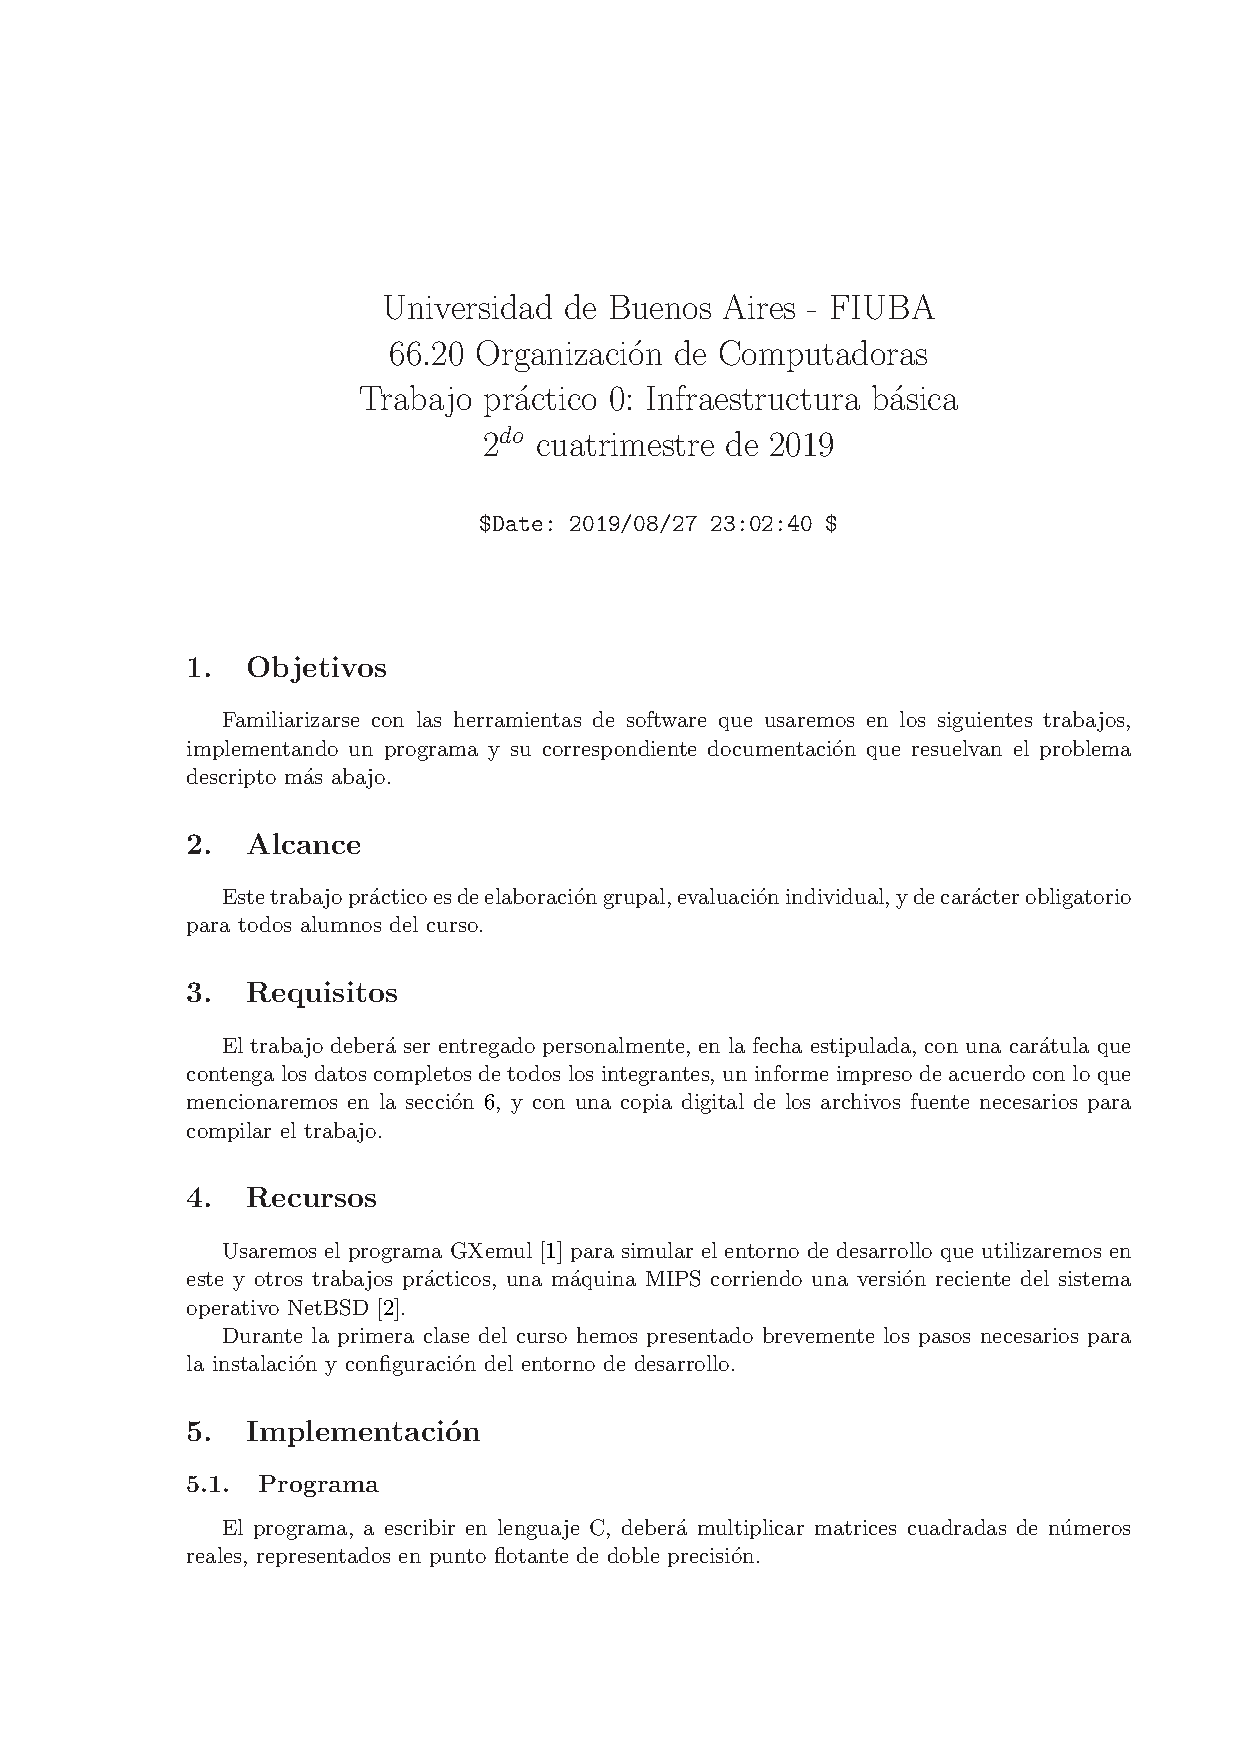
\includepdf[
    trim=20mm 30mm 10mm 25mm, clip,
    pages=1,
    frame,
    scale=.65,
    pagecommand=\section{Enunciado}
 ]{tp0-2019-2q.pdf}
\includepdf[
    trim=20mm 30mm 10mm 25mm, clip,
    pages=2-,
    frame,
    scale=.65,
    pagecommand={}
 ]{tp0-2019-2q.pdf}

\section{Solución}

\subsection{Diseño}

La solución propuesta para este trabajo comprende una serie de funciones que pueden ser clasificadas según una determinada división de responsabilidades:

\begin{itemize}
	\item \textbf{Procesamiento:} Comprende las funciones dedicadas a lectura y procesamiento de datos para obtener las matrices a multiplicar.
  \item \textbf{Buffering:} El procesamiento requiere la utilización de un buffer dinámico que almacene los valores numéricos de punto flotante de doble precisión, que primero 
  son almacenados como un array de \lstinline{char}, y luego convertidos al tipo \lstinline{double}.
  \item \textbf{Implementación de matrices:} Esta parte comprende la interfaz definida por el enunciado para la creación, impresión, multiplicación y destrucción de matrices.
  \item \textbf{Presentación:} Refiere al código generado para imprimir menús y mensajes de error.
\end{itemize}

\subsubsection{Buffering}

Este fragmento de la solución contiene las funciones \lstinline{init_buffer} y \lstinline{push}. La primer función inicializa el buffer. 
La segunda, agrega caracteres a un buffer ingresado como arugmento, manejando dinámicamente la memoria alocada por el buffer on demand.

\subsubsection{Procesamiento}

Esta parte cuenta con las siguientes funciones: 

\begin{itemize}
  \item \lstinline{get_value:} Esta función escribe sobre un puntero pasado como argumento el valor de punto flotante obtenido, correspondiente a una 'palabra' leida por \lstinline{stdin}. 
  Esta misma función se utiliza para leer el primer valor entero que indica el tamaño de la matriz cuadrada. Para esto luego se castea el valor obtenido al tipo \lstinline{size_t}.
  
  Para controlar y validar el input, la función retorna la cantidad de caracteres que leyó para obtener el valor.
	\item \lstinline{read_matrix:} Aquí se invoca las veces necesarias a la función \lstinline{get_value} para obtener los valores de cada matriz.
  En caso de llegar a whitespaces o símbolos no esperados, imprime un error que advierte que el formato del input es inválido. Las matrices las almacena en un puntero a \lstinline{matrix_t}.

  \item \lstinline{process_line:} Como bien lo indica el nombre, esta función procesa una línea de standard input. Lee el primer valor para obtener la dimensión de las matrices. 
  Por cada matriz, invoca a la inicialización de las variables de tipo \lstinline{matrix_t}, y luego a la función \lstinline{read_matrix}.
  
  Por último llama a \lstinline{matrix_multiply} para multiplicar las matrices y almacenar el resultado en un nuevo puntero a \lstinline{matrix_t}, para luego imprimir esta última matriz.
\end{itemize}


\subsubsection{Implementación de matrices}

Esta sección escencialmente implementa las interfaces propuestas por el enunciado. En particular se destacan las siguiente implementaciones:

\begin{enumerate}
	\item \lstinline{create_matrix:} Esta función requiere alocar memoria para la estructura de \lstinline{matrix_t}, y luego para el array de valores una vez conocido el tamaño de la matriz cuadrada.
  
  Por ello esta función realiza 2 memory allocation. Finalmente se inicializan los atributos de la matriz correspondientemente.
  
  \item \lstinline{destroy_matrix:} Como complemento de \lstinline{create_matrix}, esta función debe liberar la memoria alocada tanto para el array de valores como para la estructura inicializada.
\end{enumerate}

\subsubsection{Presentación}

Esta sección resuelve la mayor parte de las interacciones con el usuario del programa:

\begin{enumerate}
	\item \lstinline{argsHandler_parse_arguments:} Parseo de argumentos y ejecución de la rutina correspondiente.
  \item \lstinline{print_help, print_usage, print_options:} 
  
  Impresión de menú de ayuda y detalle de las opciones de ejecución del programa.
\end{enumerate}

\subsubsection{Main function}

La función \lstinline{main} sencillamente invoca al parseo de argumentos para imprimir menús de ayuda u opciones según corresponda. 
Sino invoca a la rutina que lee el input por \lstinline{stdin} y procesa las líneas.

\subsection{Código}

\lstinputlisting{../dynamic.c}

\lstset{
  language=bash,
  basicstyle=\small\ttfamily
}

\subsection{Compilación del programa}
Para compilar el programa se utiliza el makefile desde el directorio donde se descomprimió el entregable:
\begin{lstlisting}
$ make clean
$ make all
gcc -std=c99 -Wall -Werror -pedantic -pedantic-errors  -c dynamic.c
gcc -o dynamic dynamic.o
	
\end{lstlisting}

\section{Pruebas}

\subsubsection{Ejecución}

Para la ejecución de las pruebas generamos un script llamado \lstinline{run_tests.sh} que se encarga de, para cada caso generado, ejecutar el programa y escribit el output en un archivo.
Finalmente, se comparan los outputs contra archivos que contienen los resultados esperados, en la carpeta \lstinline{results/}.

\subsection{Casos de prueba}

Para probar nuestro programa generamos una serie de casos de prueba:

\begin{itemize}
  \item \lstinline{big_matrix_ints.txt:} Matriz de 100x100 con valores enteros
	\item \lstinline{big_matrix_doubles.txt:} Matriz de 100x100 con valores de punto flotante
  \item \lstinline{exponential_doubles_matrix.txt:} Matriz pequeña con valores de punto flotante en notación exponencial. 
  \item \lstinline{invalid_input.txt:} Prueba con input invalido. 
  \item \lstinline{simple_multiline.txt:} Prueba de input con varias líneas. 
  \item \lstinline{single_line.txt:} Prueba simple de una sola línea. 
  \item \lstinline{small_double_matrix.txt:} Prueba simple de una matriz 3x3 de doubles. 
  \item \lstinline{small_int_matrix.txt:} Prueba simple de una matriz 3x3 de integers. 
\end{itemize}

La ejecución de los casos se realiza de la siguiente manera:

\begin{lstlisting}
$ ./run_tests.sh
\end{lstlisting}

Este script de ejecución valida también la impresión del menú y de la versión del programa.

\section{Código MIPS}

\subsection{Código assembly generado para \textit{dynamic.c}}

\lstinputlisting{../dynamic.s} 

\section{Conclusiones}

Como conclusión podemos enumerar una serie de conocimientos que adquirimos y/o pusimos en práctica durante el desarrollo de este trabajo práctico.


A modo de conclusión podemos decir que en este trabajo práctico pudimos configurar y familiarizarnos con el entorno de trabajo de la materia, que emula una computadora con procesador MIPS. 
. Además adquirimos conocimiento respecto a otras herramientas útiles como ssh, scp, y diff entre otras.

\begin{itemize}
  \item Configurar y familiarizarnos con el entorno de trabajo de la materia, que emula una computadora con procesador MIPS.
	\item También pudimos observar algunas de las diferencias entre programar para un sistema operativo linux y para el netBSD que corre emulado.
	\item Empleamos comandos y herramientas útiles como ssh, scp, diff, echo, cat, entre otros.
  \item Implementamos un buffer de manejo dinámico de memoria.
  \item Utilizamos valgrind para analizar la memoria alocada durante la ejecución, detectar leaks tanto de heap como de stack, y revisar los accesos a memoria con punteros.
\end{itemize}

\end{document}
